%================ch3======================================
\chapter{Genomics Application}\label{ch:ch3}

\section{Role of Genomics in Clinical Microbiology} 
There are multiple applications for genomics in clinical
microbiology\cite{ray2003}. 
\begin{itemize}
	\item  Real-time genomics may be used to investigate infectious disease outbreaks
	\item  Bacterial genomes may be used as target sources for molecular detection, identification or genotyping.
	\item The gene content, obtained by comparison to databases such as Clusters of Orthologous Groups (\url{www.ncbi.nlm.nih.gov/COG/}) or Kyoto Encyclopedia of Genes and Genomes (\url{www.genome.ad.jp/kegg/}), may be searched for specific phenotypic traits such as virulence or antibiotic resistance markers, or deficient metabolic pathways enabling design of improved culture media.
	
	\item Antigenic epitopes detected in the deduced proteome may be
	used for serologic applications, development of monoclonal
	antibodies or development of vaccines (Figure~\ref{fig:genome}).
	\item Taxonomic description of new bacterial species.
\end{itemize}

\begin{figure}
	\centering
	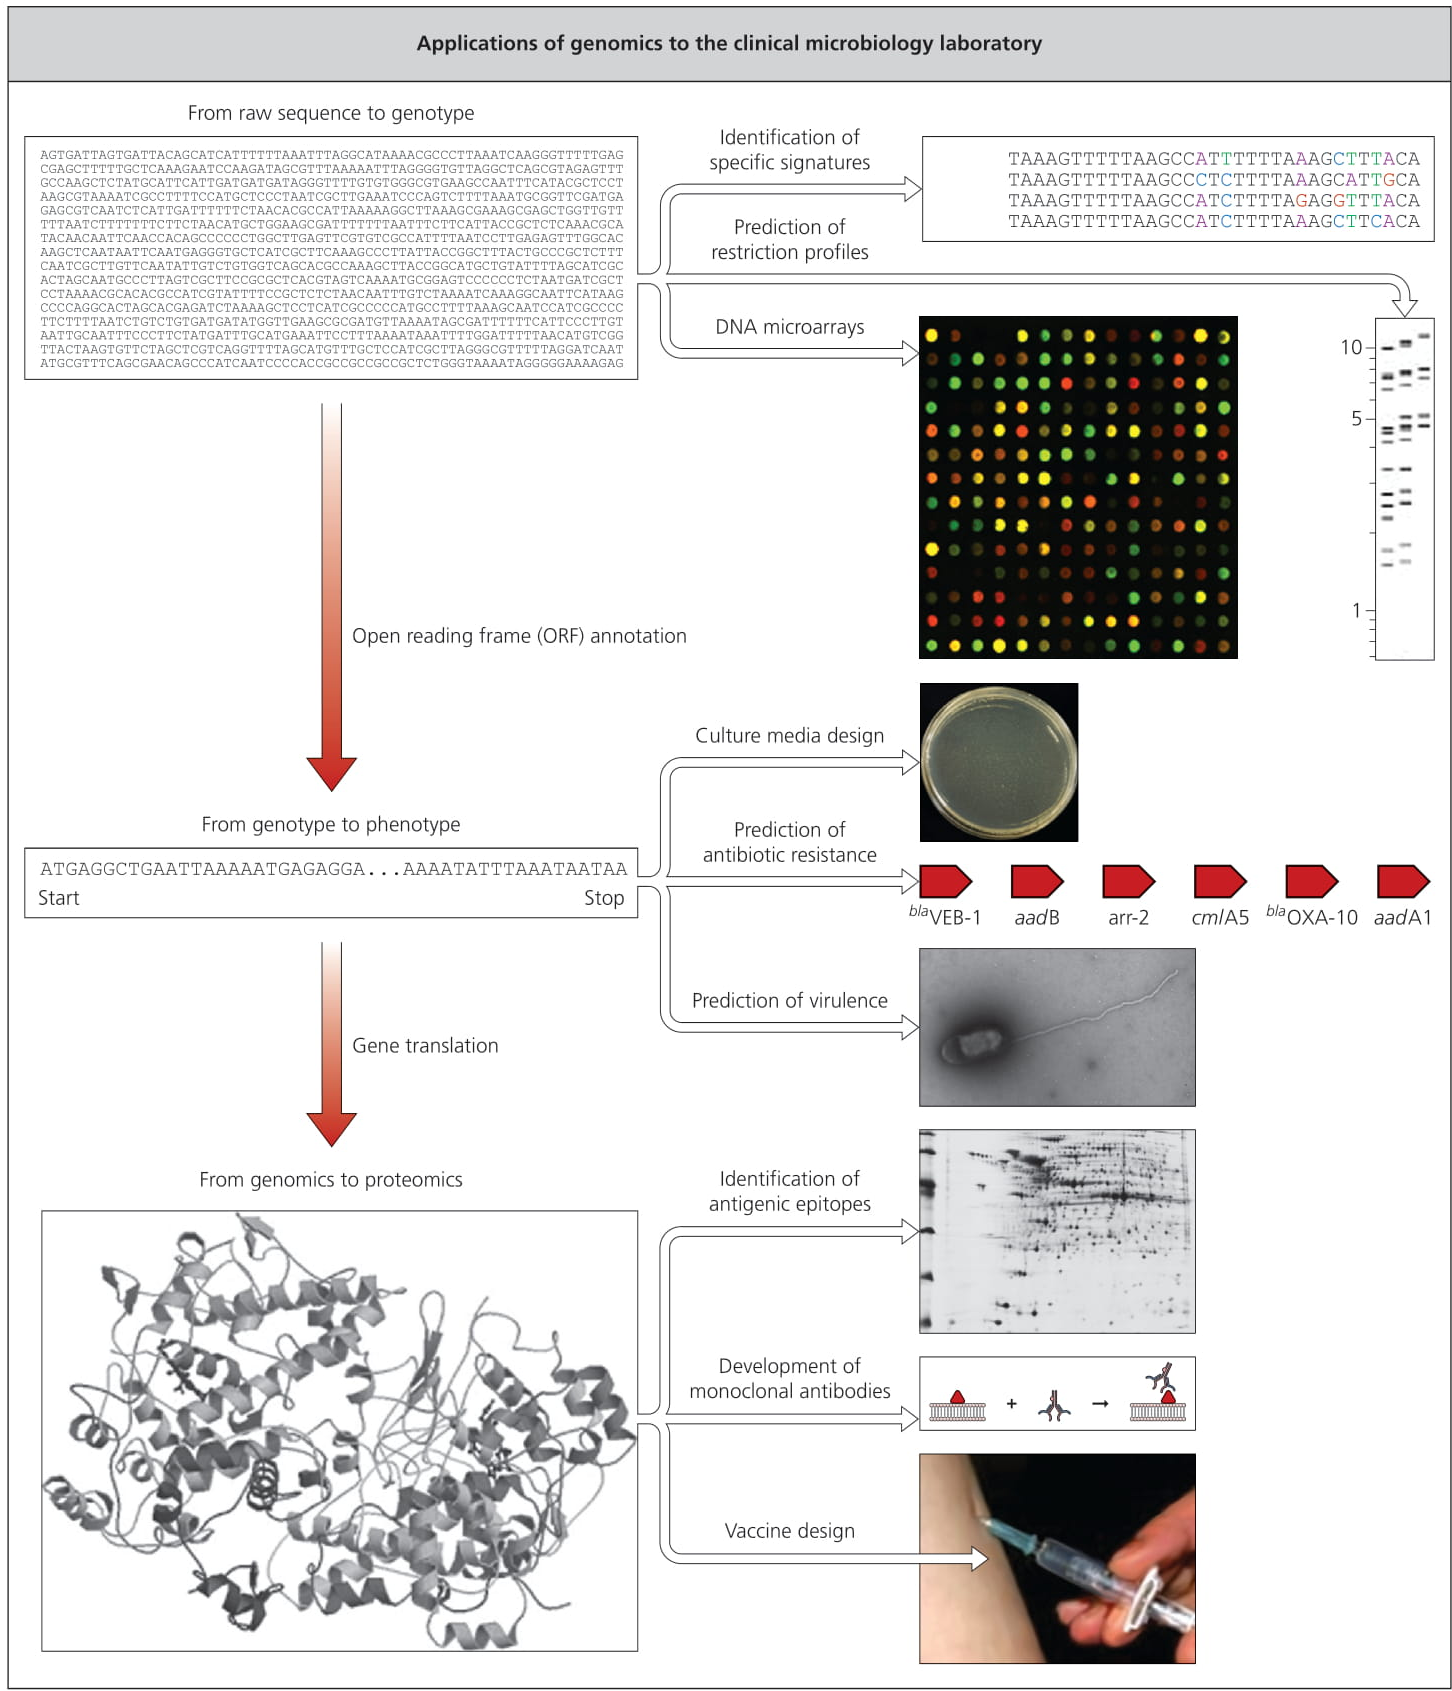
\includegraphics[width=0.9\linewidth]{backterial_genome}
	\caption{Applications of genomics to the clinical microbiology laboratory.}
	\label{fig:genome}
\end{figure} 


\section{The Clinical Applications of Genomic Technologies}
The clinical applications of genomic technologies are vast and offer opportunities to improve healthcare across the breadth of medical specialities. I will explore some of these applications in more depth this section.

\subsection{Gene discovery and diagnosis of rare monogenic disorders} 
Genomic technologies can be used by clinicians from all specialities to diagnose their patients who have high-risk genetic errors causing disease. Researchers are using these techniques to identify new genes which cause genetic disease at an astonishing rate - over 4000 diseases now have a known single genetic cause, compared to around 50 in 1990.

\subsection{Identification and diagnosis of genetic factors contributing to common disease} 
Genomic technologies are increasingly being used to understand the contribution of both rare and common genetic factors to the development of common diseases, such as high blood pressure, diabetes and cancer.

\subsection{Pharmacogenetics and targeted therapy}
Genetic information may be used to predict whether a person will respond to a particular drug, how well they will respond to that drug and whether they are likely to get any side effects from the use of a specific drug. This allows their treating team to make individualised decisions about the right drug treatment. In some cases, such as cancer, we can identify the genetic drivers of disease and then give drugs which specifically target that pathway. This is known as targeted therapy.

\subsection{Prenatal diagnosis and testing}
Genetic diseases are often devastating and may cause significant disability and even death in childhood. Prenatal diagnosis of genetic diseases allows parents to make decisions about whether to continue with the pregnancy or to allow early diagnosis and possible treatment in utero or at birth. Whilst previous approaches to prenatal diagnosis could put the pregnancy at risk, new methods using genomic technology can look directly at the DNA of the fetus from a maternal blood test, without increasing the risk of miscarriage - this is known as non-invasive prenatal testing. The use of NGS and array technology in prenatal samples is also on the increase to improve diagnostic yields in a pregnancy.

\subsection{Infectious diseases} 
Sequencing the genomes of microorganisms which cause human infection can identify the exact organism causing symptoms, help to trace the cause of infectious outbreaks, and give information as to which antibiotics are most likely to be effective in treatment.


\subsection{Personalised medicine}
As the exact DNA sequence of the genome of each human is unique to them, we will all have unique disease susceptibilities and treatment responses. Personalised medicine describes the use of our genetic information to tailor health care intervention to our own individual need.

\subsection{Gene therapy}
Gene therapy involves the administration of DNA or RNA, in order to correct a genetic abnormality, or modify the expression of genes.

\subsection{Genome editing}
Genome editing uses molecular techniques to modify the genome - genome editing can add in, cut out, or replace sections of the DNA sequence.

\subsection{Design of new antimicrobial agents and vaccines}
One of the expected benefits of genome analysis of pathogenic bacteria is in the area of human health, particularly in the design of more rapid diagnostic reagents and the development of new vaccines and antimicrobial agents. These goals have become more urgent with the continuing spread of antibiotic resistance in important human pathogens. Moreover, results from the whole-genome analysis of human pathogens has suggested that there are mechanisms for generating antigenic variation in proteins expressed on the cell surface that are encoded within the genomes of these organisms\cite{fraser2000microbial}.
These mechanisms include the following:

\begin{enumerate}
	\item slipped-strand mispairing
	within DNA sequence repeats found in 58-intergenic regions and coding sequences as described for \textit{H. influenzae2} \textit{ Helicobacter pylori26}  and \textit{M. tuberculosis27} 
	
	\item recombination between homologous genes
	encoding outer-surface proteins as described for Mycoplasma
	genitalium28, Mycoplasma pneumoniae29 and Treponema pallidum30 (Figure~\ref{fig:vac})
	
	\item clonal variability in surface-expressed proteins as described for Plasmodium falciparum31 and possibly Borrelia burgdorferi32. \cite{fraser2000microbial}
	
\end{enumerate} 

\begin{figure}
	\centering
	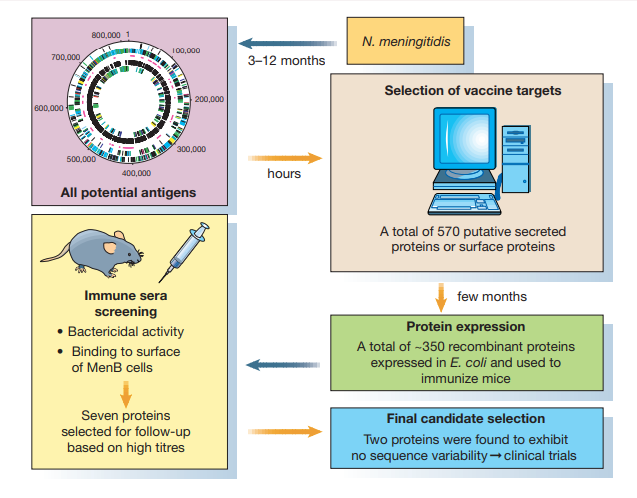
\includegraphics[width=0.9\linewidth]{vaccine}
	\caption{ Diagram depicting how complete microbial genome sequence data can accelerate vaccine development.}
	\label{fig:vac}
\end{figure} 

